\section{Redactarea 'in \LaTeX. C\^ateva sfaturi generale}
\label{sec:general}
% \label{nume} - este o eticheta pusa in contexul ultimei numerotari, in acest caz este numarul sectiunii.
% Pentru a va referi la ea, va trebui sa folositi \ref{nume}
%
% Este recomandat ca numele referintei sa indice tipul de referinta (in exemplul de mai sus, este o sectiune)


'In \LaTeX\ pute'ti redacta  rapoarte 'stiin'tifice care s'a arate impecabil. Pentru a v'a ini'tia 'in folosirea \LaTeX\ v'a recomand s'a citi'ti de exemplu un tutorial cum ar fi
{\em LaTeX Tutorial}, disponibil la 
\href{http://ece.uprm.edu/~caceros/latex/introduction.pdf}{http://ece.uprm.edu/$~$caceros/latex/introduction.pdf} 'si s'a ave'ti la 'indem\^an'a o carte mai detaliat'a, cum ar fi
{\em The Not So Short Introduction to Latex}, disponibil'a la
\href{https://tobi.oetiker.ch/lshort/lshort.pdf}{https://tobi.oetiker.ch/lshort/lshort.pdf}. 
Dac'a nu parcurge'ti o astfel de documenta'tie, atunci frazele de mai jos s-ar putea s'a va apar'a ca fiind f'ar'a sens.


\subsection{Structurarea documentului}
\label{sec:structura}
'Inainte de a scrie un raport, trebuie s'a stabili'ti cuprinsul lui. 
Dup'a fiecare comand'a de sec'tionare, scrie'ti un scurt paragraf explicativ pentru ce urmeaz'a.

\LaTeX\ ofer'a multe comenzi 'si macro-uri, dar pot fi definite 'si  unele noi. 
Este recomandat ca toate macro-urile noi definite s'a fie puse 'in preambul
('intre ultima comand'a \texttt{\string\usepackage} 'si
\texttt{\string\begin\string{document\string}}). Remarca'ti macro-urile noi definite pentru generarea acestui document ('in fi'sierul 
principal, \texttt{\string\newcommand}).

Folosi'ti automatismul \LaTeX\  pentru a face referin'te 'incruci'sate c'atre numere de sec'tiuni, ecua'tii, figuri.
Detalii g'asi'ti 'in documenta'tia recomandat'a la 'inceputul paragraful \ref{sec:general}.

Etichetele trebuie s'a fie unice, altfel la compilarea fi'sierelor vor apare {\em warnings}, iar rezultatul va avea referin'te nerezolvate, marcate cu \texttt{[?]}. {\color{red} Pentru un rezultat impecabil trebuie s'a ave'ti 
\texttt{0 Error(s), 0 Warning(s)}}.


\subsection{C\^ateva detalii}
\label{sec:detalii} 
Urmeaz'a c\^ateva detalii, despre modul de scriere al ecua'tiilor, inserare a figurilor 'si tabelelor.

\subsubsection{Ecua'tii}
Ecua'tiile sunt centrate. Vectorii se noteaz'a cu litere aldine, drepte, ca de exemplu
%                                        % nu lasati un rand liber intre text si ecuatia care continua fraza
\begin{equation}
\label{eq:produs_vectorial}
\vect{a}\times\vect{b}=\vect{c},          % se folosesc semne de punctuatie 'si in ecua'tie; aici se termina propozitia
\end{equation}
unde $\vect{a}$, $\vect{b}$, $\vect{c}$ sunt vectori reali $n$ dimensionali.

Referirea la ecua'tii se face dup'a cum urmeaz'a:
\begin{itemize}
\item Rela'tia (\ref{eq:produs_vectorial}) noteaz'a produsul vectorial dintre vectorii $\vect{a}$ 'si $\vect{b}$ cu $\vect{c}$.
\item Dar, observa'ti c'a 'in (\ref{eq:produs_vectorial}) produsul vectorial este notat cu $\times$.
\end{itemize}
'In concluzie, 'incepe'ti o propozi'tie cu cuv\^antul ``Rela'tia" sau  ``Ecua'tia" dar  nu folosi'ti cuv\^antul ``ecua'tia"
sau abrevierea  ``ec." atunci c\^and referin'ta este 'in mijlocul frazei.

Folosi'ti ``$\times$"  pentru a indica un produs vectorial, 'si ,
``$\cdot$" pentru a indica un produs scalar. La 'inmul'tirea dintre un scalar 'si un vector nu pune'ti punct, de exemplu
\begin{equation}
\label{eq:produs_scalar_vector}
\vect{y} = \alpha \vect{a},           % litere grecesti \alpha \beta \gamma \delta \Delta \omega \Omega \varphi   etc
\end{equation}
unde $\alpha \in \reale$ este un scalar real, iar $\vect{a}, \vect{y} \in \reale^n$. 'Intotdeauna trebuie s'a existe 'in text explica'tiile m'arimilor care intervin 'in rela'tiile matematice.

Indicii 'si puterile trebuie s'a fie scrise cu litere drepte atunci c\^and sunt cuvinte sau abrevieri.
De asemenea, unit'a'tile de m'asur'a, operatorii diferen'tiali 'si unitatea imaginar'a trebuie scrise cu litere drepte, ca de exemplu:
\begin{equation}
V_{\mathrm{out}} = \oint_C \vect{E}\cdot\D \vect{r} = -\frac{\D\varphi}{\D t} =  % \D este definita in preambul
4.7\,\mu\mathrm{V},
% "\," de mai sus adauga un mic spatiu intre valoare si unitatea de masura 
\end{equation}
sau
\begin{equation}
\label{eq:nabla}
\nabla\times\vect{E} = -\I \omega\mu\vect{H}.
\end{equation}
Observa'ti micul spa'tiu dintre num'ar 'si unitatea de m'asur'a. Folosi'ti
``$\varDelta$" pentru un increment infinitezimal 'si ``$\eul$" pentru num'arul lui Euler.  %\eul a fost definit in preambul
Observa'ti modul de folosire a semnelor de punctua'tie. Nu l'asa'ti r\^anduri libere 'in fi'sierele \texttt{.tex} dec\^at atunci c\^and 'incepe un paragraf nou, altfel documentul va fi pres'arat cu o mul'time de spa'tii goale. Observa'ti c'a 'in fi'sierul surs'a, dup'a ecua'tia
(\ref{eq:nabla}) nu exist'a niciun r\^and liber, iar paragraful urm'ator este, 'in consecin't'a, neindentat.

Nu folosi'ti trecerea for'tat'a la r\^and nou, cu \verb \\  dec\^at 'in situa'tii excep'tionale!

Dac'a ave'ti mai multe ecua'tii de aliniat una sub alta pute'ti folosi \texttt{eqnarray}, caz 'in care rezultatul arat'a astfel
\begin{eqnarray}
x & = & \frac{y}{z}, \\
z & = & \sum_{i=1}^n a_k,
\end{eqnarray}
sau \texttt{equation} combinat cu \texttt{array} caz 'in care rezultatul arat'a mai compact, astfel:
\begin{equation}
\begin{array}{ccl} % c - centrat, l - aliniat la stanga
x & = & \frac{y}{z}, \\
z & = & \sum_{i=1}^n a_k.
\end{array}
\end{equation}
'In primul caz toate ecua'tiile sunt numerotate dac'a nu exist'a o instruc'tiune special'a \texttt{\string\nonumber} care s'a anuleze numerotarea. 'In al doilea caz, grupul de rela'tii va avea un singur num'ar. Al doilea caz permite 'si marcarea grupului cu acolade, ca 'in exemplul urm'ator, 'in care a fost blocat'a 'si numerotarea automat'a.
\begin{equation}
\left\{
\begin{array}{ccl} % c - centrat, l - aliniat la stanga
x & = & \frac{y}{z}, \\
z & = & \sum_{i=1}^n a_k.
\end{array}  
\right. \nonumber % marcarea inchiderii - falsa; blocarea numerotarii
\end{equation}

\subsubsection{Figuri}

Figurile trebuie s'a arate ca 'in Fig.~\ref{fig:figura_exemplu}. Referirea la figuri se face astfel:
\begin{itemize}
\item Figura \ref{fig:figura_exemplu} $\ldots$ atunci c\^and propozi'tia 'incepe cu cuv\^antul
``Figura".
\item 'In mijlocul unei propozi'tii, se scrie "'in Fig.~\ref{fig:figura_exemplu} pute'ti observa ....".
\end{itemize}

\begin{figure}[ht]  %preferinte: mai intai h - here apoi t- top, htb-, b-bottom
\centering
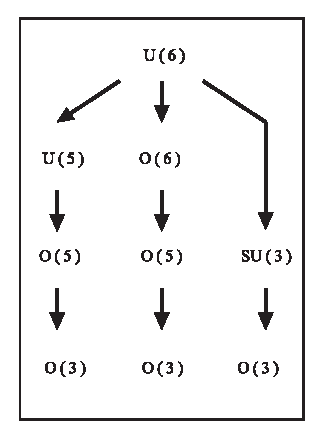
\includegraphics{tex_files/figs/authorfig1.eps}
%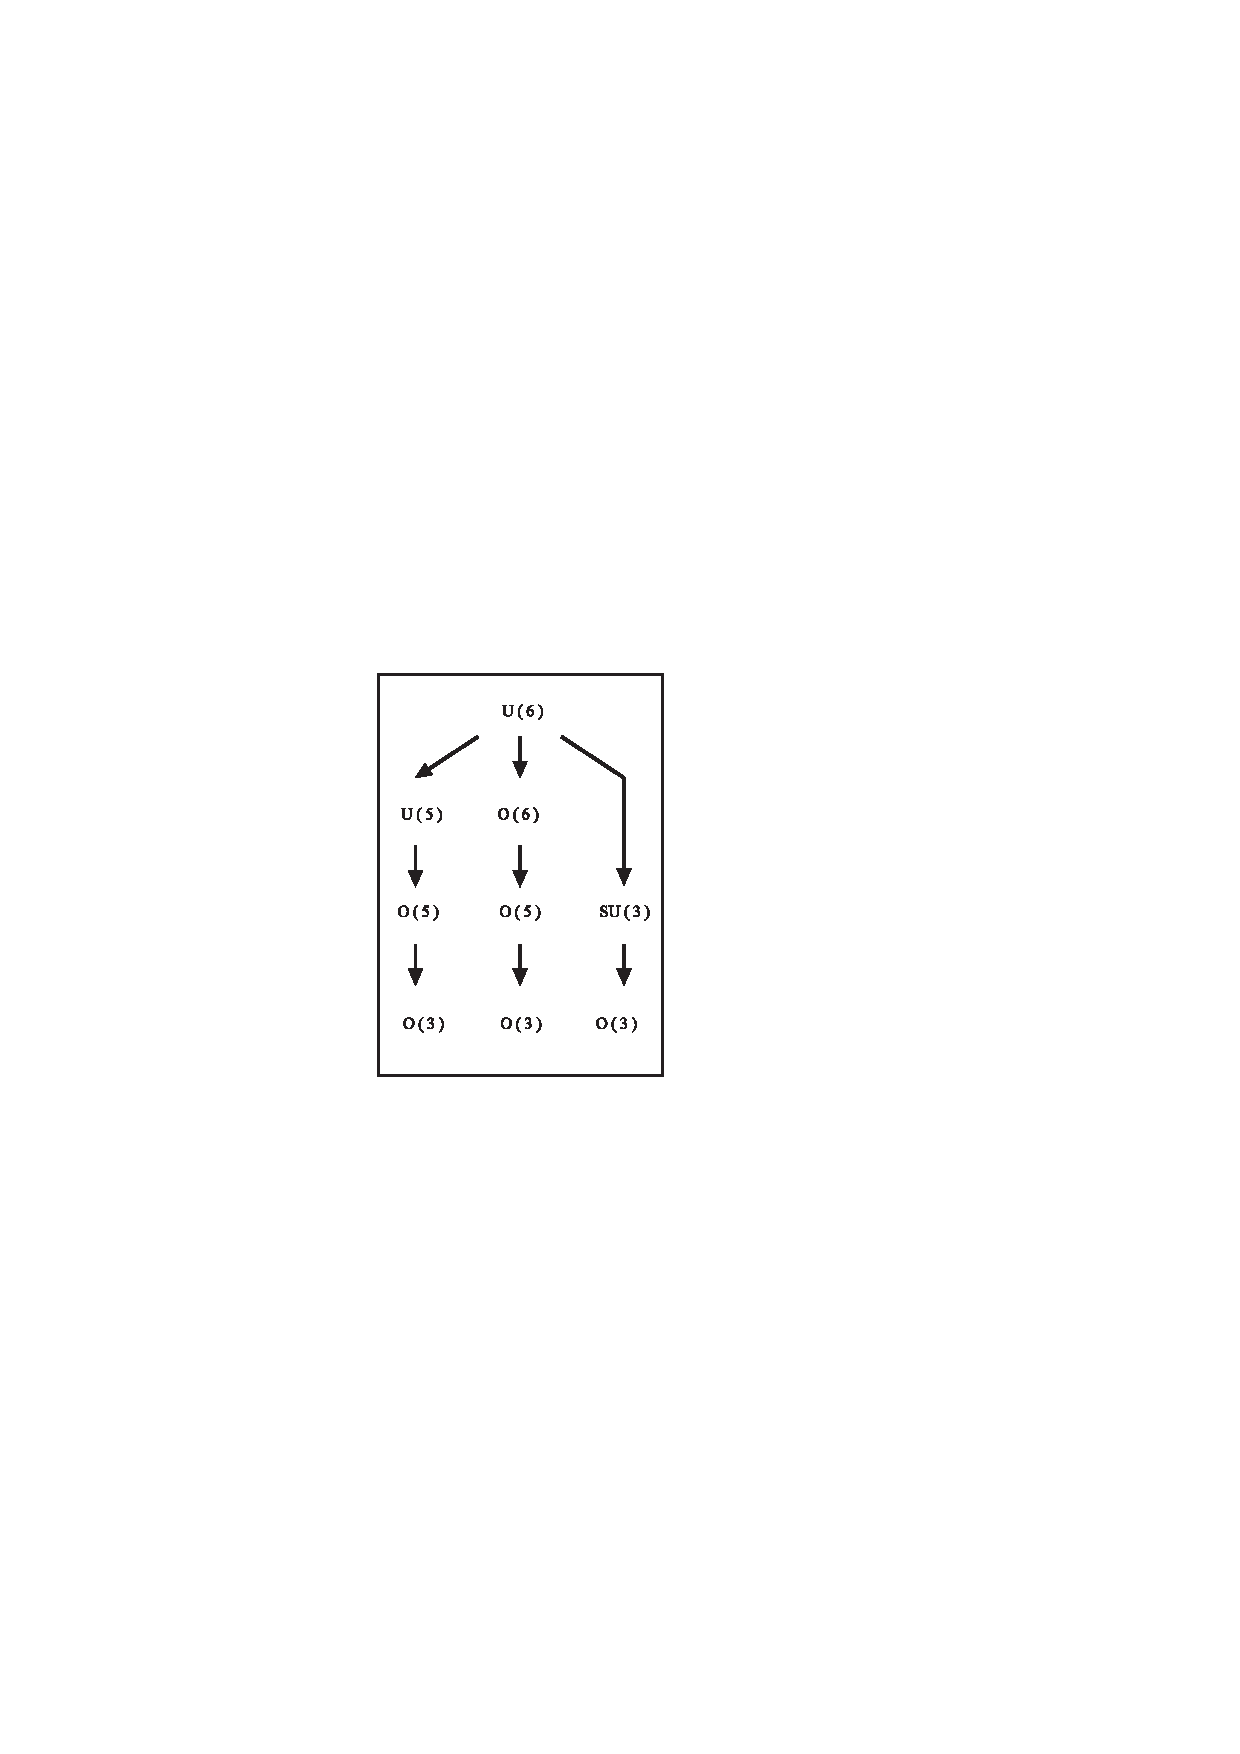
\includegraphics{tex_files/figs/authorfig1.jpeg}
\caption{O figur'a are 'intotdeauna un titlu scris sub ea, iar 'in text exist'a o referire la ea. G'asi'ti 'in text referirea la aceast'a figur'a.}
\label{fig:figura_exemplu}       
\end{figure}

Dac'a este necesar, pute'ti pune dou'a figuri una l\^ang'a alta, fie cu un titlu comun ca 'in Fig.\ref{fig:figura_exemplu2}, fie cu titluri separate ca 'in Fig.\ref{fig:figura_exemplu3} 'si Fig.\ref{fig:figura_exemplu4}. Titlurile au semne de punctua'tie!
\begin{figure}[ht]  %h - here, dar puteti pune si t-top, b-bottom
\begin{minipage}{0.5\textwidth}
\centering
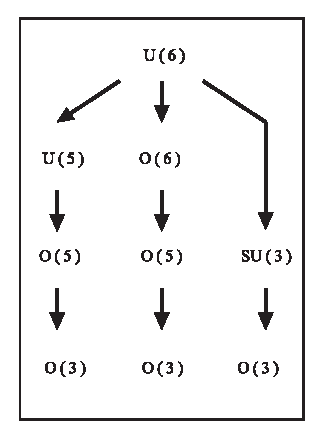
\includegraphics{tex_files/figs/authorfig1.eps}
%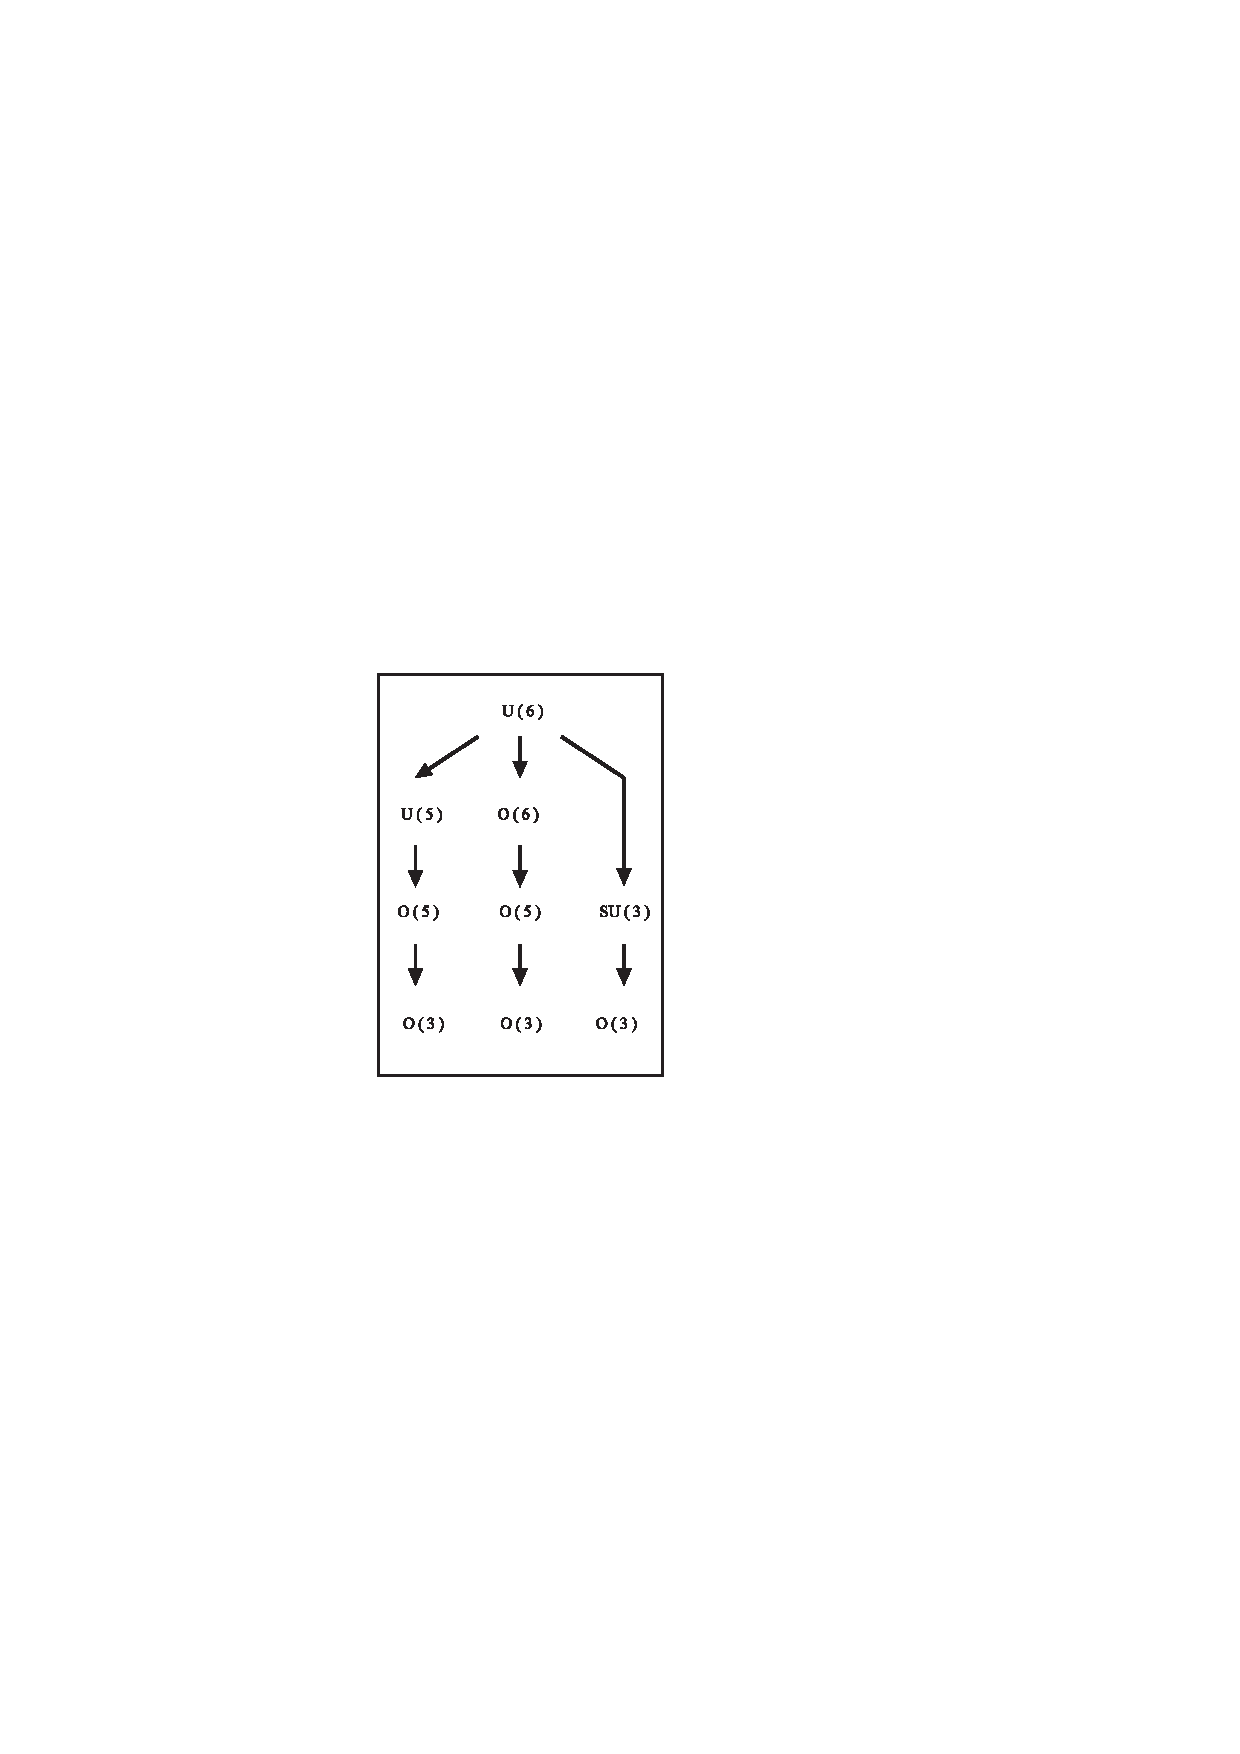
\includegraphics{tex_files/figs/authorfig1.jpeg}
\end{minipage}
\begin{minipage}{0.5\textwidth}
\centering
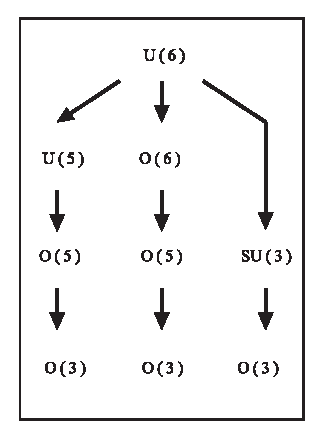
\includegraphics{tex_files/figs/authorfig1.eps}
%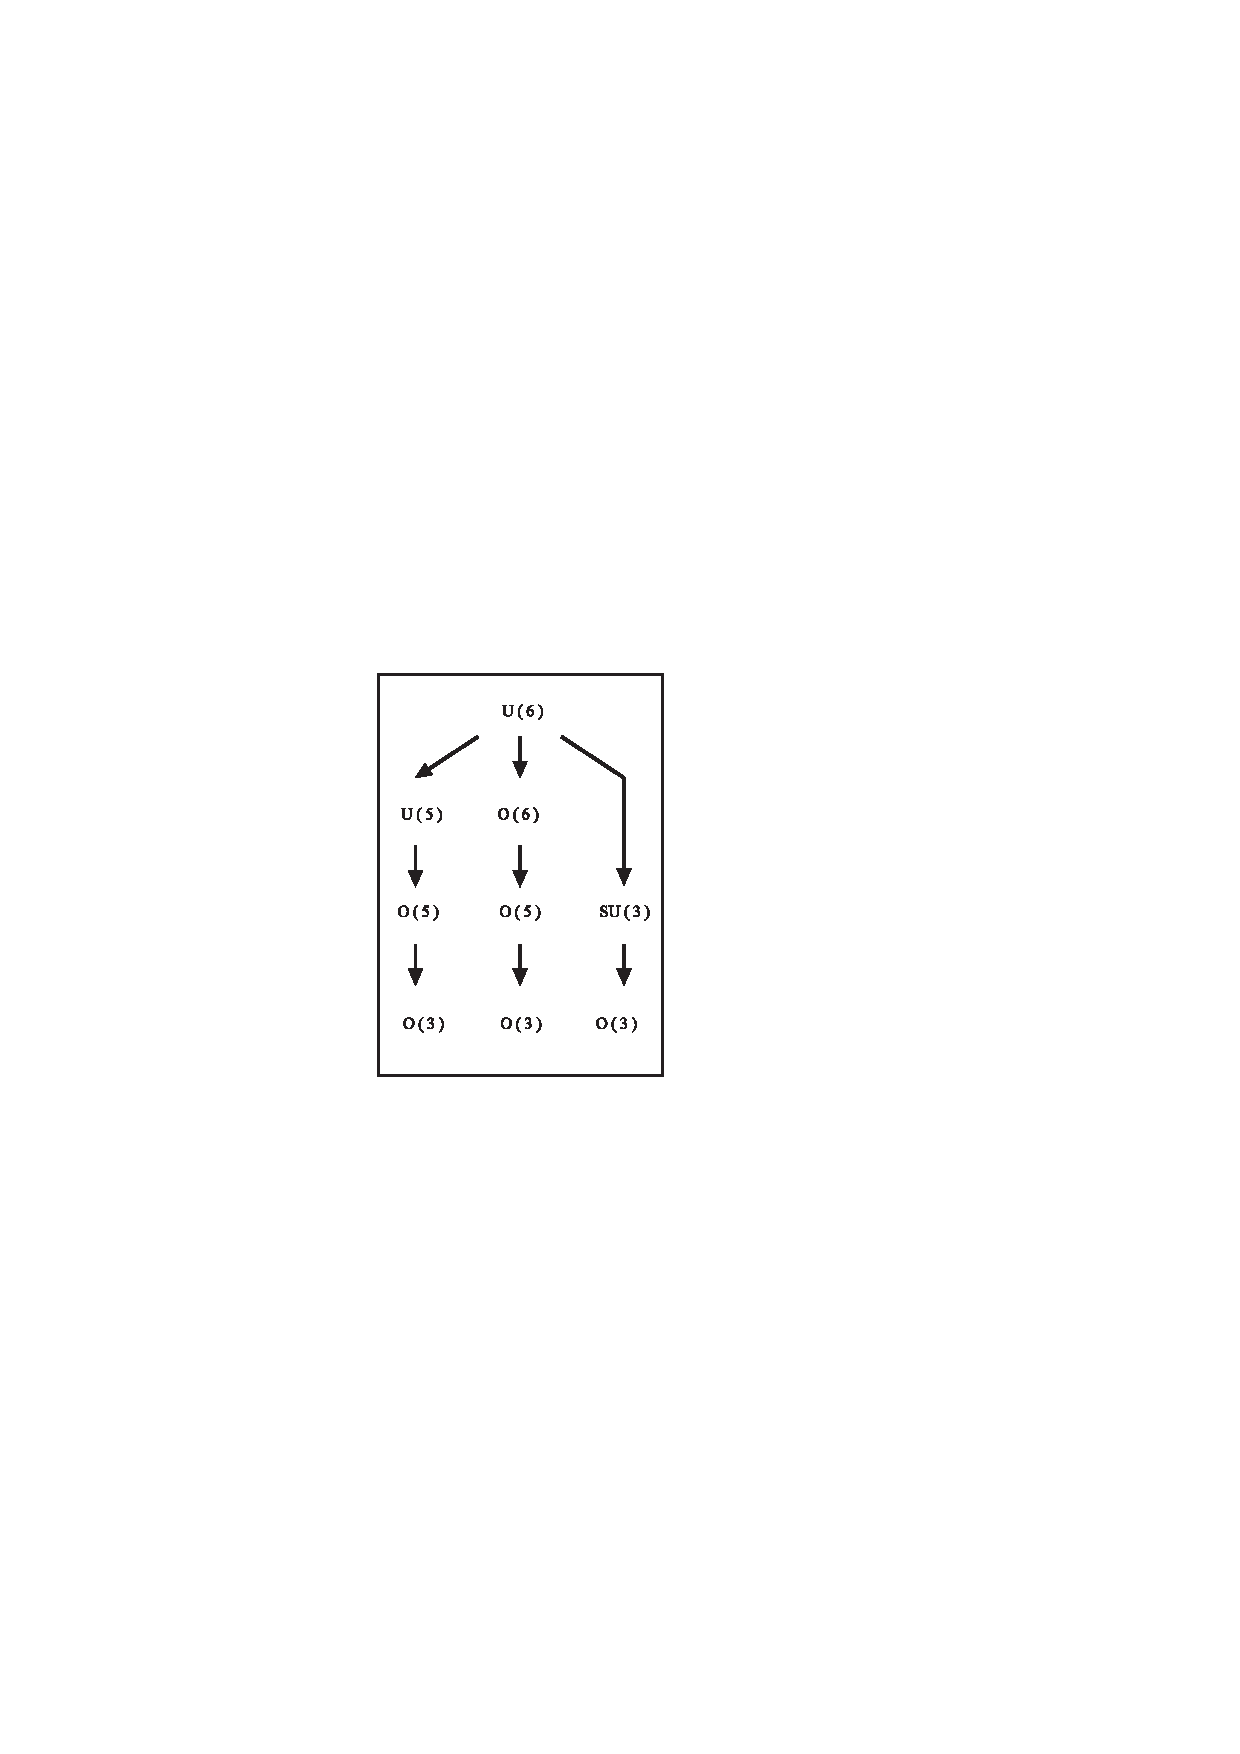
\includegraphics{tex_files/figs/authorfig1.jpeg}
\end{minipage}
\caption{Titlu comun, dar trebuie explicat ce e 'in st\^anga 'si ce e 'in dreapta.}
\label{fig:figura_exemplu2}       
\end{figure}

\begin{figure}[ht]  %preferinte: mai intai h - here apoi t- top, htb-, b-bottom
\begin{minipage}{0.5\textwidth}
\centering
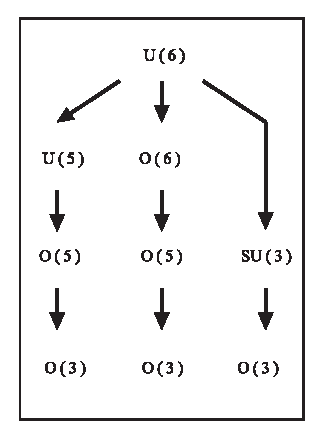
\includegraphics{tex_files/figs/authorfig1.eps}
%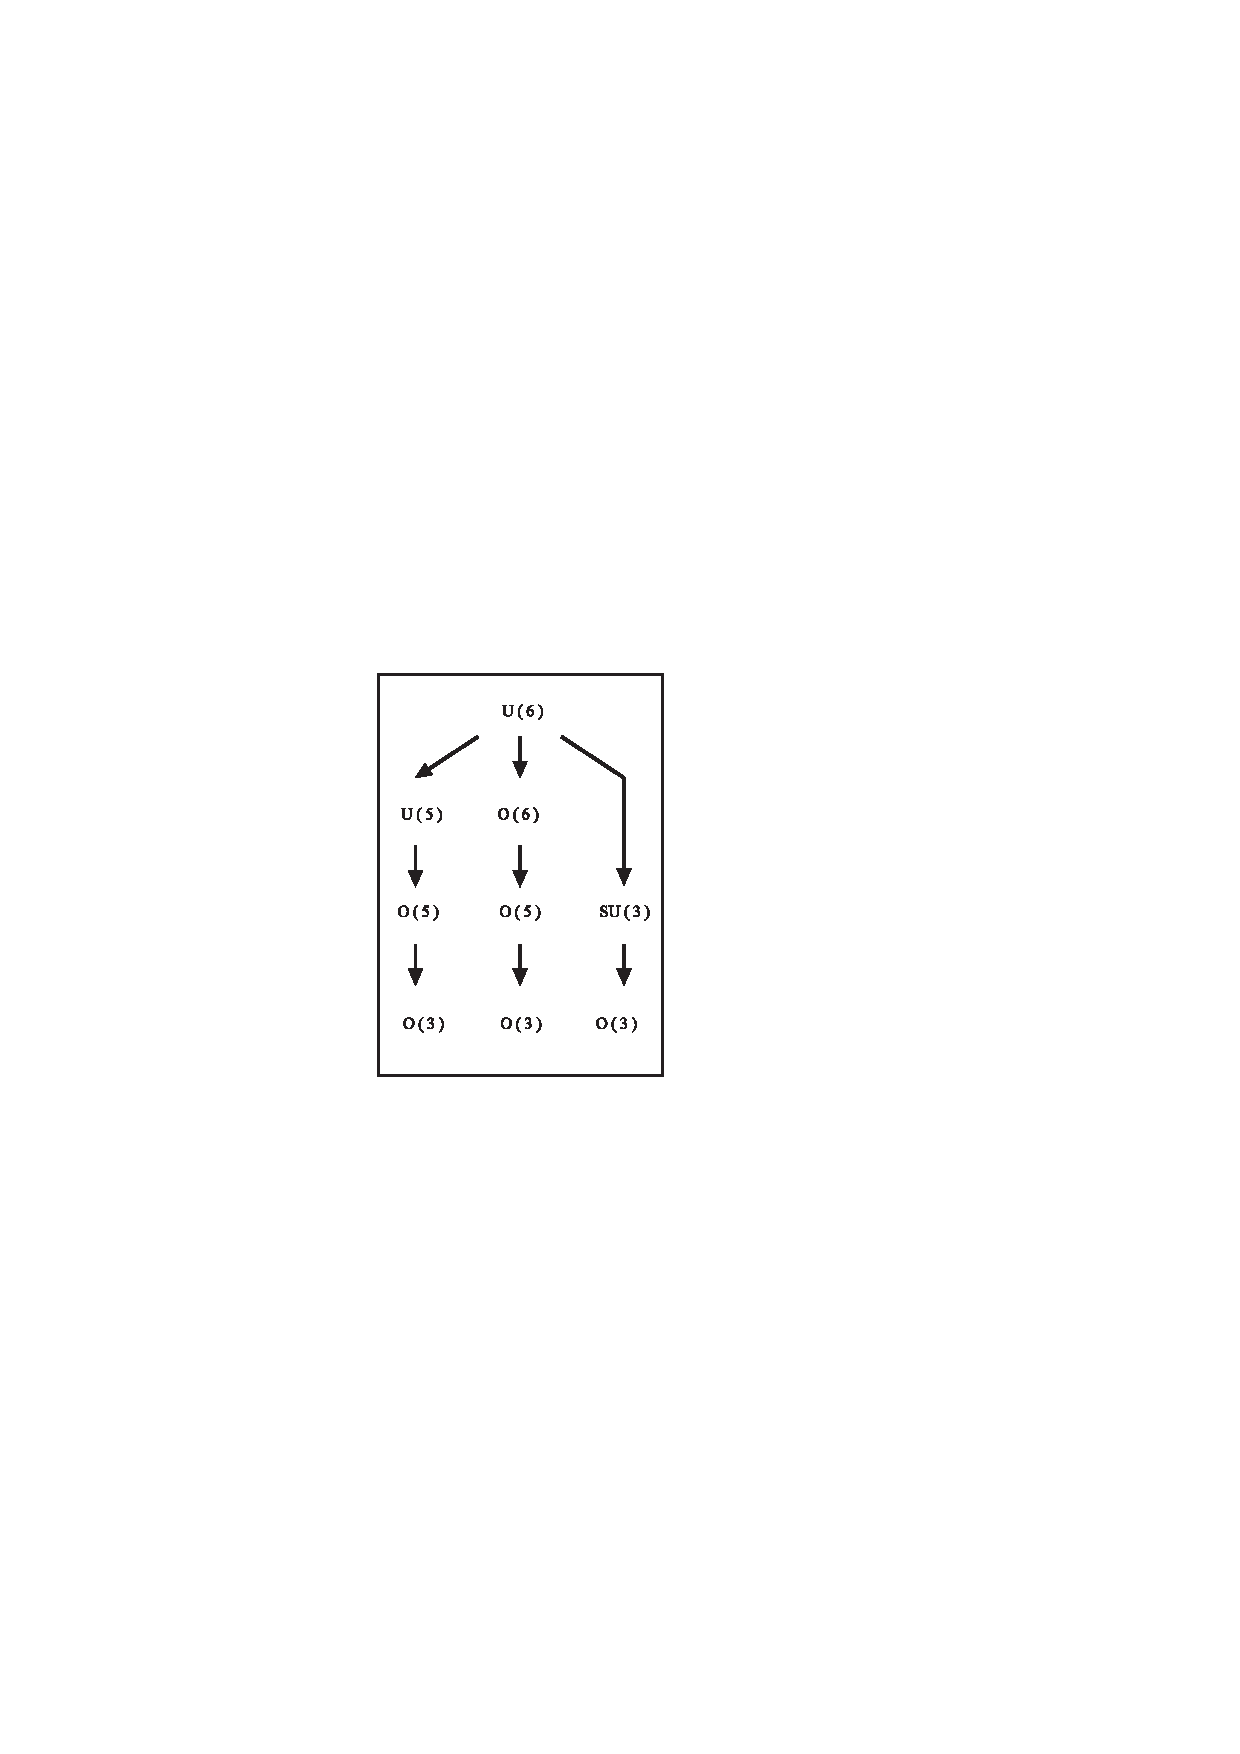
\includegraphics{tex_files/figs/authorfig1.jpeg}
\caption{Titlu st\^anga.}
\label{fig:figura_exemplu3}       
\end{minipage}
\begin{minipage}{0.5\textwidth}
\centering
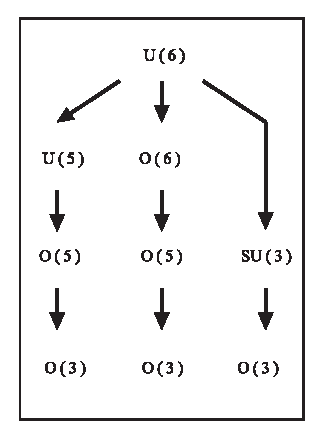
\includegraphics{tex_files/figs/authorfig1.eps}
%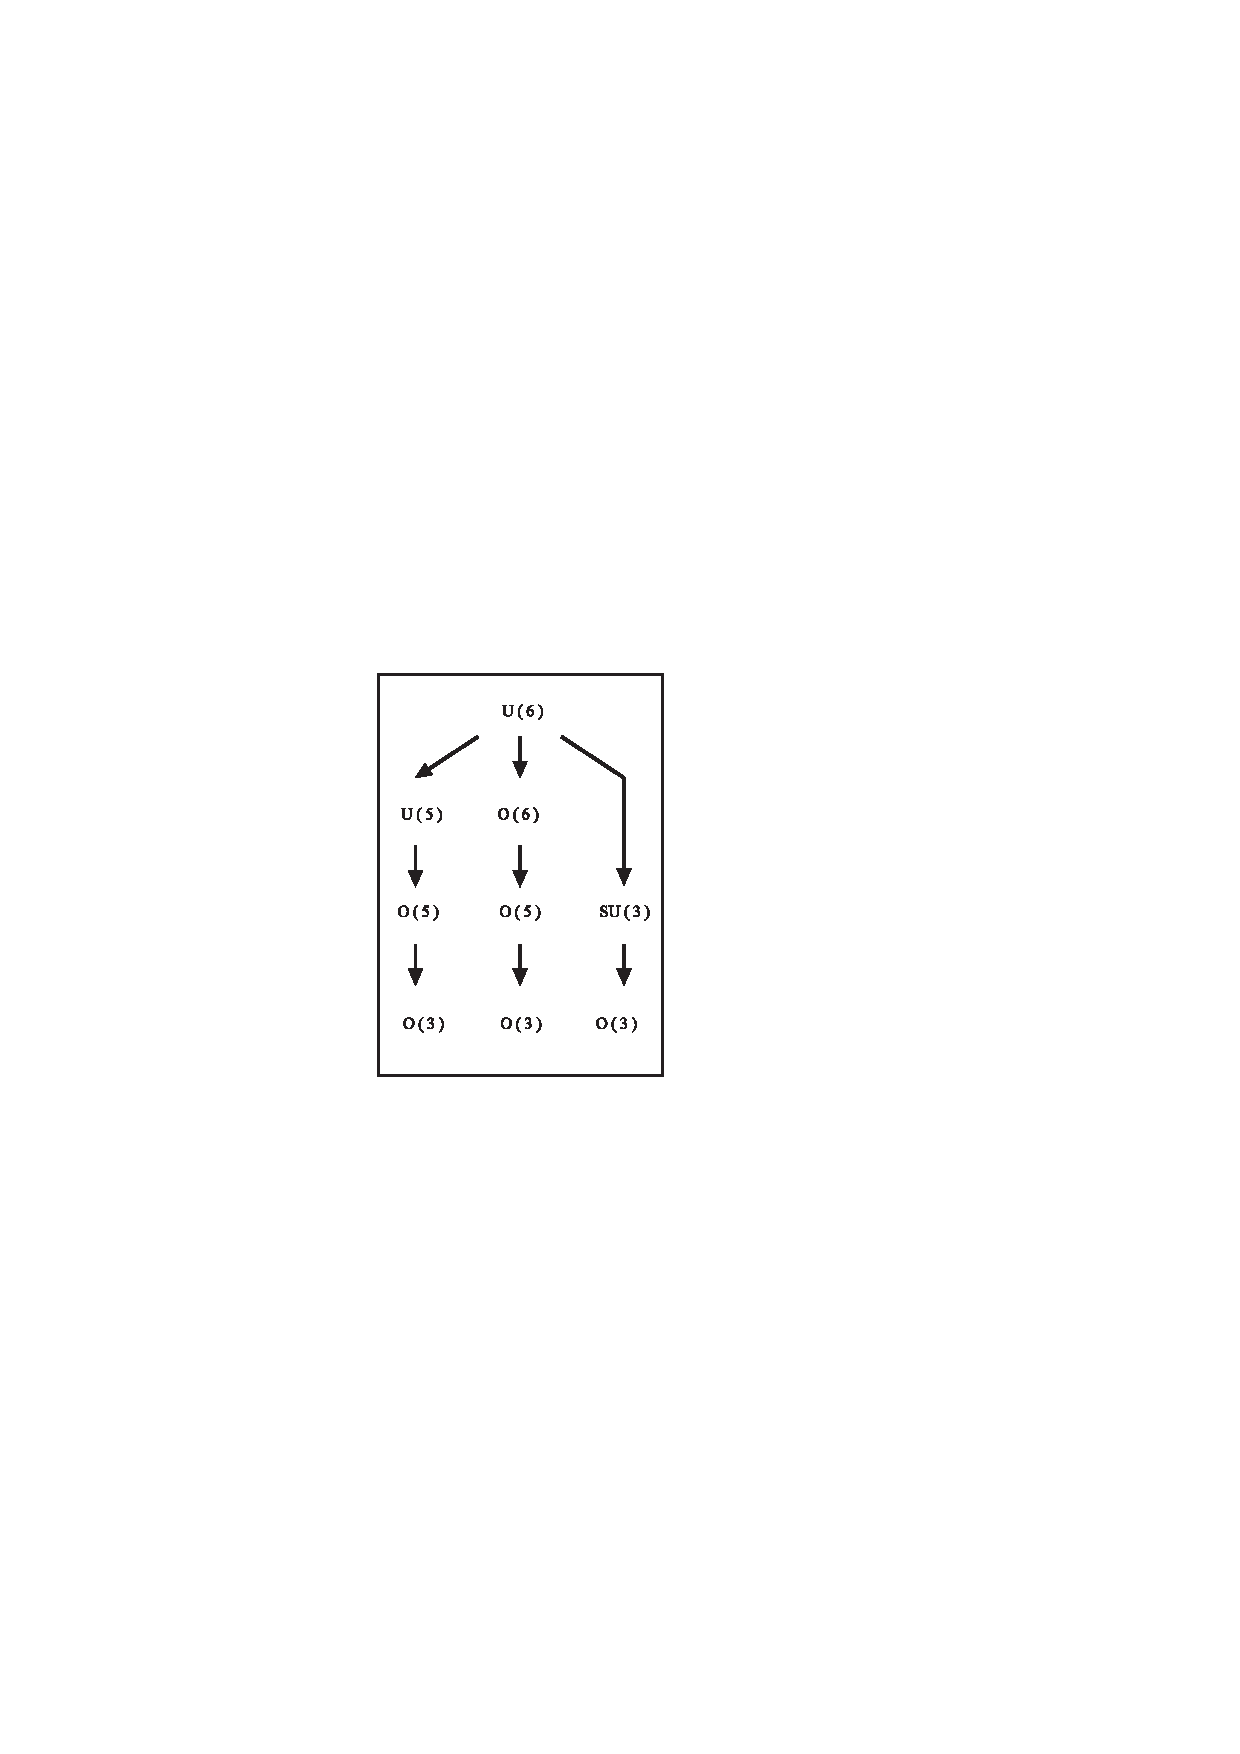
\includegraphics{tex_files/figs/authorfig1.jpeg}
\caption{Titlu dreapta.}
\label{fig:figura_exemplu4}       
\end{minipage}

\end{figure}

Pot fi folosite diferite formate de figuri, vede'ti documenta'tia\footnote{'In acest raport figurile sunt {\tt .eps}, iar documentul pdf a fost generat trec\^and prin formatul {\tt .ps}. 
'In Windows se poate folosi ca mediul de lucru TeXnicCenter 
\href{http://www.texniccenter.org/}{http://www.texniccenter.org/}, iar sub Linux, texstudio \href{http://www.texstudio.org/}{http://www.texstudio.org/}. 
Pentru lucrul sub linux pute'ti g'asi util fi'sierul {\tt Makefile} pe care 'il g'asi'ti de asemenea 'in arhiva de fi'siere. Citi'ti 'si observa'tiile din fi'sierul {\tt README1.txt}}.

Pentru figuri de calitate bun'a, este bine s'a folosi'ti imagini vectoriale \\ % rand liber fortat pentru ca link-ul e prea lung 
\href{http://www.techterms.com/definition/vectorgraphic}{http://www.techterms.com/definition/vectorgraphic}.

S-ar putea uneori s'a dori'ti s'a realiza'ti o figur'a de calitate mai bun'a prin folosirea unui limbaj, vede'ti de exemplu
\href{https://en.wikipedia.org/wiki/PGF/TikZ}{https://en.wikipedia.org/wiki/PGF/TikZ}.
Un exemplu de astfel de figur'a este 
Fig.\ref{fig:tikz}. Figura este preluat'a de la \\
\href{http://tex.stackexchange.com/questions/158668/nice-scientific-pictures-show-off}{http://tex.stackexchange.com/questions/158668/nice-scientific-pictures-show-off}.

\begin{figure}[ht]  %preferinte: mai intai h - here apoi t- top, htb-, b-bottom
\centering
%% Generated with LaTeXDraw 2.0.8
% Tue Nov 02 10:50:27 EET 2010
% \usepackage[usenames,dvipsnames]{pstricks}
% \usepackage{epsfig}
% \usepackage{pst-grad} % For gradients
% \usepackage{pst-plot} % For axes
\scalebox{1} % Change this value to rescale the drawing.
{
\begin{pspicture}(0,-4.5892186)(13.021875,4.6092186)
\definecolor{colormyred}{rgb}{0.8,0.0,0.0}
\definecolor{colormygreen}{rgb}{0.2,0.6,0.0}
\definecolor{colormyblue}{rgb}{0.0,0.2,0.8} % albastru
\psline[linewidth=0.04cm,arrowsize=0.1cm 2.0,arrowlength=2,arrowinset=0.4]{->}(0.9,-0.32)(11,-0.32)
\psline[linewidth=0.04cm,arrowsize=0.1cm 2.0,arrowlength=2,arrowinset=0.4]{<-}(5.3,4.3)(5.3,-4.5)
\psline[linewidth=0.08cm,linecolor=colormygreen](0.0,-2.0892189)(12.34,4.0107813)
\psline[linewidth=0.08cm,linecolor=colormyred](2.46,-4.5692186)(11.7,4.5107813)
\psframe[linewidth=0.06,linecolor=colormyblue,linestyle=dashed,dash=0.16cm 0.16cm,dimen=outer](6.78,0.55078125)(5.3,-0.32)
\psframe[linewidth=0.06,linecolor=colormyblue,linestyle=dashed,dash=0.16cm 0.16cm,dimen=outer](7.66,1.2507813)(6.78,0.55078125)
\psframe[linewidth=0.06,linecolor=colormyblue,linestyle=dashed,dash=0.16cm 0.16cm,dimen=outer](8.4,1.7107812)(7.66,1.2507813)
\usefont{T1}{ptm}{m}{n}
\rput(11.1,0.02078125){$x_1$}
\usefont{T1}{ptm}{m}{n}
\rput(4.9414062,4.2407813){$x_2$}
\usefont{T1}{ptm}{m}{n}
\rput(10.651406,4.420781){\color{colormyred}$\Delta_1$}
\usefont{T1}{ptm}{m}{n}
\rput(12.241406,3.3807812){\color{colormygreen}$\Delta_2$}
\usefont{T1}{ptm}{m}{n}
\rput(5.8,0){${\mathbf{x}^{(0)}}$}
\usefont{T1}{ptm}{m}{n}
\rput(7.2,0.8){${\mathbf{x}^{(1)}}$}
%\usefont{T1}{ptm}{m}{n}
%\rput(8.7,2){${\mathbf{x}^{(2)}}$}
\end{pspicture} 
}
  % trebuie sa compilati prin postscript
  \begin{tikzpicture}

\draw[thick,-latex] (0,0,0) -- (4,0,0) node[anchor=north east]{$y$};
\draw[thick,-latex] (0,0,0) -- (0,7.5,0) node[anchor=north west]{$z$};
\draw[thick,-latex] (0,0,0) -- (0,0,5) node[anchor=south]{$x$};
\filldraw (0,6,0) circle (1.75pt) node[left,font=\small]{$P(0,0,b)$};

\fill[top color=gray!50!black,bottom color=blue!10,middle color=gray,shading=axis,opacity=0.25] (0,0) circle (2cm and 0.5cm);
\fill[left color=gray!50!black,right color=blue!50!black,middle color=gray!50,shading=axis,opacity=0.25] (2,0) -- (2,4) arc (360:180:2cm and 0.5cm) -- (-2,0) arc (180:360:2cm and 0.5cm);
\fill[top color=blue!90!,bottom color=blue!2,middle color=blue!30,shading=axis,opacity=0.25] (0,4) circle (2cm and 0.5cm);
\draw (-2,4) -- (-2,0) arc (180:360:2cm and 0.5cm) -- (2,4) ++ (-2,0) circle (2cm and 0.5cm);
\draw[densely dashed] (-2,0) arc (180:0:2cm and 0.5cm);

\draw[densely dashed] (-2,2.8) arc (180:0:2cm and 0.5cm);
\draw[densely dashed] (-2,2.6) arc (180:0:2cm and 0.5cm);
\draw[thick] (-2,2.8) arc (180:360:2cm and 0.5cm);
\draw[thick] (-2,2.6) arc (180:360:2cm and 0.5cm);
\draw[thick, orange] (2,2.6) -- (3,2.6);
\draw[thick, orange] (2,2.8) -- (3,2.8);
\draw[thick,-latex] (2.8,4) -- (2.8,2.8);
\draw[thick,-latex] (2.8,1.6) -- (2.8,2.6);
\draw[thick,latex-] (2.8,0) -- (2.8,1.2) node[above] {$z$};
\draw [dashed] (0,6)--(3,6);
\draw[thick,latex-] (2.8,6) -- (2.8,4.5)node[below]{$b-z$};
\node at (3.5,2.7) [anchor=east]{$dz$};
\node at (2,1.5) [anchor=east]{$\rho_v\ (C/m^3)$};
\draw (-2,0) to[dim above=$L$,color=orange] (-2,4) ;

\coordinate (vec1) at (30:1);
\draw[-latex,thick] (0,0) -- (vec1)node[midway,sloped, above, inner sep=1] {$a$};
\draw[ultra thick,-latex,blue] (0,6,0) -- (0,7,0) node[right] {$\mathbf{E}$};
     \end{tikzpicture}   
\caption{Figura generat'a cu comenzi Tikz}
\label{fig:tikz}
\end{figure}

\subsubsection{Tabele}

Informa'tia de tip tabelar, trebuie prezentat'a ca 'in
Tabelul~\ref{tab:exemplu_tabel}.

\begin{table}[ht]  %preferinte: mai intai h - here apoi t- top, htb-, b-bottom
\centering
\caption{Titlurile tabelelor se pun deasupra tabelelor.}
\label{tab:exemplu_tabel}       % eticheta trebuie sa fie unica
%
% Informatia propriu zisa urmeaza
%
\begin{tabular}{|p{2cm}||c|l|r|p{3cm}|}  \hline  % l = left, c = center, r = right
Metoda & Dimensiune $n$ & Info1 & Info2 &Obs.  \\ \hline \hline
Metoda A & $10^3$  & 22 (19--25) & AAA& aaa\\
Metoda B & $3 \cdot 10^{4}$ & 21 & BB & bb\\
Metoda C & $10^6$  & 21--22 & CCCC& ccccc\\  \hline
\end{tabular}
\end{table}

\subsubsection{Liste}

Pentru listele numerotate se folose'ste \verb|enumerate|
ca de exemplu:
\begin{enumerate}
\item{Text aaa.}
\begin{enumerate}
\item{Text bbb.}
\item{Text ccc.}
\end{enumerate}
\item{Text ddd.}
\end{enumerate}

Pentru listele nenumerotate se folose'ste \verb|itemize| ca de exemplu:
\begin{itemize}
\item{Text 'in list'a nenumerotat'a, referire la Tabelul~\ref{tab:exemplu_tabel}.}
\begin{itemize}
\item{Text 'in list'a nenumerotat'a - x.}
\item{Text 'in list'a nenumerotat'a - y.}
\end{itemize}
\item{Text 'in list'a nenumerotat'a - z.}
\end{itemize}

Pentru o list'a de defini'tii sau nota'tii pute'ti folosi \verb|description|, ca de exemplu
\begin{description}
\item[$\vect{E}$]{Intensitatea c\^ampului electric [V/m] - m'arime fizic'a vectorial'a, ce caracterizeaz'a local starea c\^ampului electric 'in vid. }
\item[$\vect{H}$]{Intensitatea c\^ampului magnetic [A/m] - m'arime fizic'a vectorial'a, ce caracterizeaz'a local starea c\^ampului magnetic 'in vid. }
\end{description}


